\documentclass[a4paper,10pt]{article} 

\usepackage{amsmath}
\usepackage{amssymb}
\usepackage{color}
\usepackage{graphicx}
\usepackage{listings}
\usepackage{lmodern}
\usepackage{mdframed}
\usepackage{url}
\usepackage[utf8]{inputenc}
\usepackage[T1]{fontenc}
\usepackage{graphicx}
\usepackage{caption}
\usepackage{subcaption}
\usepackage{hyperref}
\usepackage{geometry}
\usepackage{booktabs}
\usepackage{float}
\usepackage{cite}
\usepackage{xcolor}
\usepackage{pgfgantt}
\usepackage{rotating}
\usepackage{tikz}

\geometry{margin=1in}

\newcommand{\BlackBox}{\rule{1.5ex}{1.5ex}}

\definecolor{blue}{rgb}{0,0,0.8}
\definecolor{dkgreen}{rgb}{0,0.6,0}
\definecolor{gray}{rgb}{0.5,0.5,0.5}
\definecolor{mauve}{rgb}{0.58,0,0.82}

\lstset
{
   basicstyle=\ttfamily\footnotesize,
   language=C++,
   numbers=right,
   numberstyle=\color{gray},
   showtabs=true,
   breaklines=true,
   breakatwhitespace=true,
   captionpos=bottom,
   keywordstyle=\color{blue},
   commentstyle=\color{dkgreen},
   stringstyle=\color{mauve},
   frame=single
}

\mdfsetup
{
   skipabove=\topskip,
   skipbelow=\topskip,
   leftmargin=2em,
   rightmargin=2em
}


\title
{
   
\includegraphics[width=12cm]{up_logo.png} \\
   \vspace{2cm}
   \textbf{COS700 Research Proposal} \\ 
   \vspace{0.5cm}
   \textbf{Diagnosing and Repairing XAI Fragility: SAM-Optimised Rules for Cancer Drug Response} \\ 
   \vspace{0.5cm}
    Angelique Breedt u23542838 \\
    Bahiya Hoosen u22598546 \\
    Hawa Ibrahim u20418494 \\
    Melisa Ledwaba u19296950 \\
    Sakhile Manzi u26838002 \\
    \vspace{0.5cm}
   \textbf{Supervisors}: \\ Prof. Nelishia Pillay \\ Dr. Nyathi Thambo  
}

\author{}
\date{}
\begin{document}

\maketitle

\newpage
\linespread{1.25}

\section*{Abstract}
Deep Neural Networks achieve state-of-the-art predictive performance in cancer pharmacogenomics,
particularly for drug sensitivity prediction using high-dimensional genomic data. However, their
opaque black-box nature limits clinical adoption: clinicians cannot easily verify whether predictions
are grounded in genuine oncogenic biology or merely exploit learned statistical shortcuts, a
vulnerability known as the Clever Hans effect. This study proposes a Red Explainable Artificial
Intelligence (XAI) diagnostic pipeline that treats post-hoc explainability as an active model
interrogation tool rather than a justification mechanism. Using the Genomics of Drug Sensitivity in
Cancer (GDSC) dataset and the biologically informed DeepCCDS architecture, the pipeline applies
Sharpness-Aware Minimisation (SAM) to steer the model toward flatter loss landscape minima. Symbolic
if-then rules are extracted using a single-objective Genetic Algorithm and a multi-objective
Non-Dominated Sorting Genetic Algorithm II (NSGA-II), and evaluated for fidelity, comprehensibility,
and stability through a unified PROMETHEE II analysis, non-parametric Mann--Whitney U testing, and Gene
Set Enrichment Analysis (GSEA). The study hypothesises that landscape-aware regularisation will reduce
the generalisation gap and yield rules that are statistically simpler, more faithful to the model's
decision logic, and more strongly enriched in known oncogenic pathways than those from an unregularised
baseline.

\section*{Keywords}
Explainable AI (XAI), Red XAI, Cancer, Precision Oncology, Genomics of Drug Sensitivity in Cancer, GDSC, Sharpness-Aware Minimisation (SAM), Generalisation Gap, Evolutionary Algorithms

\newpage

\section{Introduction}
% -------------------------------------------------------
% ASSIGNED TO: \textcolor{green}{Person 1}
% -------------------------------------------------------
% INSTRUCTION: Keep existing content. Add the following:
% (1) A formal objectives list at the end of this section (see below).
% (2) Convert all first-person constructions to third person throughout.
% -------------------------------------------------------

Deep Neural Networks (DNNs) have achieved state-of-the-art predictive accuracy in cancer
genomics, particularly in tasks of predicting drug sensitivity using high-dimensional datasets such
as the Genomics of Drug Sensitivity in Cancer (GDSC) database \cite{Yang2013,Baptista2021}.
Despite this predictive power, DNNs operate as black-box models whose internal logic is opaque
to clinicians that utilise their predictive outputs to make life-determining decisions \cite{Arrieta2020}.
Consequently, their adoption in high-stakes clinical environments is hindered \cite{Arrieta2020, Klauschen2024}
by what this study defines as the \textit{Interpretability-Regularisation Gap}: the tension where highly
accurate, complex black-box models rely on sharp, irregular loss landscapes that produce fragile,
easily manipulated explanations, whereas intrinsically interpretable models lack the flexibility
needed to capture highly non-linear biological relationships.

Explainable Artificial Intelligence (XAI) addresses this by extracting understandable symbolic
rules from trained models \cite{Yedjour2024}, but the quality of these explanations is inseparable
from the health of the underlying model. When a DNN overfits its training data, learning spurious
correlations and dataset artefacts rather than genuine biological signal, a phenomenon known as
the ``Clever Hans'' effect takes hold \cite{Anders2022, Pahde2023, Samek2017}. The dominant
``Blue XAI'' paradigm compounds these challenges by prioritising user-facing justifications over
rigorous model auditing \cite{Biecek2024}. This project is instead grounded in ``Red XAI'', which
fosters a culture of model interrogation and debugging \cite{Biecek2024}, introducing a diagnostic
pipeline that uses a model's generalisation gap as a measurable indicator of explanation fragility.

The remainder of this proposal is structured as follows. Section 2 formally states the research
questions and hypothesis. Section 3 provides the theoretical foundation. Section 4 details the
experimental methodology. Section 5 presents the project timeline.

% -------------------------------------------------------
% NEW CONTENT REQUIRED (NICOG Slide 5 / COS700 Slide 21)
% Add the following objectives list:
% -------------------------------------------------------

\subsection*{Objectives}

% ADD: Formal objectives list using measurable verbs as required by the NICOG workshop guidelines.
% Suggested text (edit as needed):
The objectives of this study are:
\begin{enumerate}
    \item To establish a measurable overfitting baseline using the DeepCCDS architecture trained without regularisation on the GDSC dataset and to quantify the resulting generalisation gap.
    \item To evaluate whether Sharpness-Aware Minimisation (SAM) regularisation reduces the generalisation gap and produces a flatter loss landscape relative to the Adam-optimised baseline.
    \item To compare the fidelity, comprehensibility, and stability of symbolic if-then rules extracted by a Genetic Algorithm and NSGA-II from both the baseline and SAM-regularised models.
    \item To determine whether rules extracted from the SAM-regularised model show statistically significant improvement in PROMETHEE II outranking scores over baseline rules using Mann--Whitney U tests.
    \item To assess whether SAM-optimised rules show greater enrichment in established KEGG oncogenic pathways than baseline rules, as verified through GSEA pathway enrichment analysis.
\end{enumerate}

\section{Problem Statement}
% -------------------------------------------------------
% ASSIGNED TO: \textcolor{green}{Person 1}
% -------------------------------------------------------
% INSTRUCTION: Keep existing content. Add scope and limitations
% paragraph at the end (marked in red below).
% Convert first-person to third person throughout.
% -------------------------------------------------------

Currently, there is no standardised diagnostic framework that uses a model's generalisation gap
as a predictor of explanation quality. While regularisation is known to improve accuracy, research
exploring how optimisers like Sharpness-Aware Minimisation (SAM) can be used to smooth the
explanation landscape to produce rules that are faithful and comprehensible is limited
\cite{Dombrowski2022, Springer2024}. Without a ``Red XAI'' audit linking model health to rule quality,
clinicians risk relying on explanations that may be mathematically convenient but biologically
fraudulent \cite{Longo2024}.

The primary research question is as follows: to what extent can the generalisation gap serve as a
diagnostic indicator of explanation fragility, and can SAM be used to improve the fidelity and
comprehensibility of rules extracted using evolutionary algorithms?

This breaks down into four sub-research questions:

\begin{enumerate}
    \item \textbf{Correlation}: Is there a statistically significant correlation between a model's generalisation gap and the rule explosion (complexity versus fidelity) observed in extracted symbolic rules?
    \item \textbf{Regularisation Impact}: How does the transition from standard Adam to SAM-based optimisation affect the stability and sharpness of the model's error landscape, and the stability of its explanations?
    \item \textbf{Multi-Criteria Validation}: To what degree do SAM-optimised rules outrank baseline rules when evaluated through the PROMETHEE II multi-criteria framework?
    \item \textbf{Biological Alignment}: Do the rules extracted from a regularised model show higher enrichment in KEGG/Enrichr pathways compared to rules from an overfitted baseline?
\end{enumerate}

The hypothesis is that applying SAM regularisation to a neural network trained on GDSC genomic
data will reduce the generalisation gap by converging on flatter minima, resulting in symbolic rules
that are statistically simpler, more accurately aligned to the black-box logic of the model (higher
fidelity), and more consistently aligned with known biological pathways (higher biological validity)
than those produced by an unregularised baseline \cite{Foret2021, Li2018, Springer2024, Yedjour2024}.

% -------------------------------------------------------
% NEW CONTENT REQUIRED (COS700 Slide 21)
% -------------------------------------------------------

\subsection*{Scope and Limitations}

\textcolor{red}{
% ADD: Scope and limitations paragraph as required by proposal guidelines.
% Suggested text (edit as needed):
This study is scoped to the following boundaries. The neural network architecture is fixed to
DeepCCDS \cite{Wu2025} and is not subject to architectural optimisation. The primary dataset is
GDSC with LN IC\textsubscript{50} as the drug response metric; the study does not extend to
clinical patient data or real-time deployment contexts. The rule extraction pipeline operates on
discretised tabular genomic features and does not address image-based or multi-modal data
modalities. The regularisation intervention is limited to SAM as a replacement for the Adam
optimiser; other regularisation strategies such as dropout or L2 weight decay are not evaluated as
primary interventions. Statistical comparisons are conducted between the baseline and
SAM-regularised conditions only; the study does not benchmark against all possible optimisers.
Biological verification is limited to KEGG and Enrichr pathway databases as accessed through
GSEApy; wet-lab experimental validation is outside the scope of this project.
}

\section{Literature Study}
\label{sec:literature}

\subsection{Explainable AI (XAI)}
% -------------------------------------------------------
% ASSIGNED TO: \textcolor{green}{Person 2}
% -------------------------------------------------------
% INSTRUCTION: Keep existing 3.1 content (ante-hoc/post-hoc, Blue/Red XAI).
% ADD the new subsection 3.1.2 below (marked in red) — this is the
% primary gap identified by the supervisor.
% Convert first-person to third person throughout.
% -------------------------------------------------------

Explainable Artificial Intelligence encompasses a suite of techniques designed to make the
decision-making processes and predictions of complex AI models transparent and comprehensible
to human users (\textcolor{red}{verify citation}) \cite{}. Interpretability and explainability are distinct concepts in AI
\cite{Arrieta2020}: interpretability (or transparency) describes the extent to which a model's
internals naturally make sense to a human observer, while explainability is a process where a
model provides specific details to clarify its functioning and decision-making. Based on this
distinction, AI models can be classified into ante-hoc models (interpretable by design, e.g.\
decision trees, linear regression) and post-hoc techniques (applied to already-trained black-box
models to extract information) \cite{Arrieta2020}.

\subsubsection{Blue XAI vs Red XAI}

\cite{Biecek2024} categorise XAI based on the goals of the explanations into two cultures: Blue
XAI, which focuses on justifying decisions to build trust with end users, and Red XAI, which is
oriented toward developers who use explanations as active diagnostic tools to explore, validate,
and debug models. Table~\ref{tab:bluered} summarises the differences.

\begin{table}[H]
\centering
\caption{Comparison between Blue XAI and Red XAI, adapted from \cite{Biecek2024}.}
\label{tab:bluered}
\begin{tabular}{p{2.5cm}p{5cm}p{5cm}}
\toprule
\textbf{Feature} & \textbf{Blue XAI} & \textbf{Red XAI} \\
\midrule
Core Goal & Responsible, legal, trust, and ethical issues & Research on data, exploring models, and debugging \\
Target Audience & Lay users, customers, or patients & Power users, AI developers, and researchers \\
Explanation Type & Prioritises simplicity and comprehensibility & Prioritises faithfulness to the model and data \\
Primary Intent & Justify why a specific decision was made & Question the model, spot bugs, and extract knowledge \\
\bottomrule
\end{tabular}
\end{table}
\noindent
This project is rooted in the Red XAI culture, using evolutionary algorithms as a diagnostic and
research tool rather than a mere justification mechanism \cite{Biecek2024, Yedjour2024}.

% -------------------------------------------------------
% NEW CONTENT REQUIRED — PRIMARY SUPERVISOR FEEDBACK GAP
% (NICOG Slide 4: "State of the art approaches for problem")
% -------------------------------------------------------

\subsubsection{State-of-the-Art Post-Hoc XAI Methods}

\paragraph{SHAP (SHapley Additive exPlanations)}
SHAP unifies several additive feature-attribution methods under a single game-theoretic framework,
which treats each input feature like a player in a cooperative game and fairly shares out the credit
for a prediction among them, assigning each feature a Shapley value that quantifies its marginal
contribution to an individual prediction \cite{Lundberg2017}. It satisfies desirable properties such as
local accuracy and consistency, and has efficient model-specific variants such as TreeSHAP and
DeepSHAP. However, SHAP produces continuous, instance-level attributions, that is, a numeric importance
score for each feature on a single prediction rather than a discrete yes/no rule: it reports which genes
mattered for one prediction, not a generalisable decision rule that can be audited globally or expressed
as a discrete gene set for cross-referencing against KEGG pathways. Most critically for this project,
attribution-based methods of this kind have been shown to produce visually plausible explanations even
for models with randomised weights \cite{Adebayo2018}, so a SHAP explanation of an overfitted model can
look indistinguishable from that of a well-generalised one; SHAP therefore cannot detect the Clever Hans
behaviour this pipeline targets. Adversarial work, meaning deliberately crafted inputs or training
procedures designed to fool an explanation method, has further shown that SHAP can be manipulated to
conceal biased model behaviour \cite{Slack2020}. SHAP is predominantly deployed in Blue-XAI practice,
prioritising end-user justification over model interrogation.

\paragraph{LIME (Local Interpretable Model-Agnostic Explanations)}
LIME explains an individual prediction by sampling perturbed instances around it and fitting a sparse,
proximity-weighted linear surrogate (a simple linear model fitted only in the local region around the
prediction), yielding local feature importances \cite{Ribeiro2016}. Because the explanation is a local
linear approximation, it is inherently per-instance rather than global, and its faithfulness degrades
where the underlying decision surface is highly non-linear. The method is also unstable: small changes
to the perturbation neighbourhood can produce qualitatively different explanations
\cite{AlvarezMelis2018}, and in high-dimensional genomic feature spaces meaningful local neighbourhoods
become sparse, undermining the sampling strategy. Like SHAP, LIME is vulnerable to adversarial
manipulation that hides discriminatory behaviour \cite{Slack2020}, and its continuous attributions are
not directly verifiable against discrete biological pathways. LIME is thus predominantly a Blue-XAI tool
for per-prediction justification.

\paragraph{Layer-wise Relevance Propagation (LRP)}
LRP explains a prediction by back-propagating the model output and redistributing it backwards as a
relevance signal, a share of the prediction assigned to each input, onto the input features, producing a
heatmap, a colour-coded map of which inputs mattered most \cite{Bach2015,Samek2017}. While effective for
visualising salient inputs, it yields continuous relevance maps rather than auditable symbolic rules and
remains local to individual predictions. Most importantly for this project, LRP is the very instrument
through which the Clever Hans problem has been demonstrated: Pahde et al.~\cite{Pahde2023} apply LRP to
overfitted models and show it attributes high relevance to biologically incoherent or artefactual
features the model has latched onto. LRP therefore functions here as a witness to the fragility being
diagnosed rather than as a competing rule-extraction method.

\paragraph{Integrated Gradients}
Integrated Gradients attributes a prediction to its input features by accumulating gradients along a
straight-line path from a baseline input to the actual input, satisfying the completeness and
sensitivity axioms, formal guarantees that the attributions sum to the prediction and that any feature
which changes the output receives non-zero importance, that naive gradient saliency (reading the model's
raw input gradients directly) violates \cite{Sundararajan2017}. Although axiomatically stronger than
these vanilla gradient methods, it shares their core limitations: the output is a continuous,
instance-level attribution rather than a global rule, the result depends on the often-arbitrary choice
of baseline, and the path integral, the accumulation of gradients along that path, is sensitive to the
smoothness of the model's decision boundary. This last property is precisely the sharp-loss-landscape
pathology that the SAM intervention in this project is designed to correct, meaning Integrated Gradients
is most fragile exactly where model health is poorest.

\paragraph{Anchors}
Anchors is the closest state-of-the-art method to the approach taken here: rather than continuous
attributions, it produces high-precision if-then rules, where an ``anchor'' is a set of feature
conditions that locally guarantees the prediction to a user-specified precision \cite{Ribeiro2018}. This
rule-like, human-readable output is more aligned with clinical auditability than attribution heatmaps.
However, anchors are inherently local: one rule is generated per instance, with no global rule set
describing the model's overall logic, and the precision guarantee holds only in the neighbourhood of
each instance, so it need not generalise across the heterogeneous cancer subtypes in GDSC. Anchors also
optimises only for precision and coverage; it does not expose fidelity and comprehensibility as explicit
competing objectives, cannot produce a Pareto front of trade-off solutions, and therefore cannot feed
the PROMETHEE II multi-criteria ranking that structures this project's evaluation.
\\
The limitations of these SOTA methods motivate the use of evolutionary rule extraction in this project.
Unlike SHAP, LIME, LRP, and Integrated Gradients, which produce continuous feature-attribution scores
that cannot be directly verified against biological pathways in a discrete, auditable form, evolutionary
algorithms extract global symbolic if-then rules that can be explicitly evaluated for fidelity,
comprehensibility, and biological validity \cite{Yedjour2024}. Unlike Anchors, the GA and NSGA-II
pipelines optimise rule quality as explicit objectives across the full GDSC dataset rather than locally
per instance, and their outputs are directly compatible with the PROMETHEE II multi-criteria ranking
framework \cite{Yedjour2024}. Furthermore, and most critically, none of the SOTA methods described above
can detect Clever Hans behaviour: Adebayo et al.~\cite{Adebayo2018} demonstrated that popular attribution
methods including SHAP-style approaches produce visually plausible explanations even for models that have
memorised noise, because their outputs are largely independent of model parameters. This project's Red
XAI pipeline addresses this directly by auditing model health before any explanation is extracted
\cite{Biecek2024}. Table~\ref{tab:sota_comparison} provides a structured comparison.

\begin{table}[H]
\centering
\small
\caption{Structured comparison of state-of-the-art post-hoc XAI methods against the evolutionary
rule-extraction approach adopted in this project.}
\label{tab:sota_comparison}
\begin{tabular}{p{1.9cm}p{1.7cm}p{1.0cm}p{1.5cm}p{1.3cm}p{1.6cm}p{1.1cm}}
\toprule
\textbf{Method} & \textbf{Output} & \textbf{Scope} & \textbf{Auditable Rules} & \textbf{Fidelity Opt.} & \textbf{Bio. Verifiable} & \textbf{Red XAI} \\
\midrule
SHAP & Continuous scores & Local & No & No & Indirect & No \\
LIME & Continuous scores & Local & No & No & Indirect & No \\
LRP & Heatmap & Local & No & No & Indirect & No \\
Integrated Gradients & Continuous scores & Local & No & No & Indirect & No \\
Anchors & Rule (local) & Local & Partial & No & Indirect & Partial \\
\textbf{GA + NSGA-II (Ours)} & \textbf{Symbolic rules} & \textbf{Global} & \textbf{Yes} & \textbf{Yes} & \textbf{Direct (GSEA)} & \textbf{Yes} \\
\bottomrule
\end{tabular}
\end{table}

\noindent
Beyond these post-hoc methods, a distinct but related family known as explanation-guided training
modifies the training objective itself rather than explaining a fixed model after the fact. Examples
include Right for the Right Reasons \cite{Ross2017}, contextual-decomposition penalisation
\cite{Rieger2020}, adversarial training on explanations \cite{Tang2022}, and robust-explanation
objectives such as R2ET \cite{Chen2022}, REGEX \cite{Li2023}, and the Clever-Hans-specific pruning
method EGEM \cite{Linhardt2024}. These methods place the explanation directly into the loss function, in
some cases requiring human-annotated ground-truth explanations or expensive second-order gradients. They
are the nearest methodological neighbour to the approach proposed here and are revisited in the critical
analysis (Section~\ref{ssub:critical-analysis}), where their relationship to the explanation-agnostic,
geometry-only intervention used in this project is examined.

\subsection{Cancer Medicine and the Shift to Precision Pathology}
Cancer is a mixed group of diseases that can be hematologically (blood) related or 
tumour related \cite{NCI}. 
They are all characterised by their uncontrolled cellular growth that is triggered by 
genetic mutations and epigenetic changes (environmental factors) alterations 
\cite{NCI}. Traditionally, treatment of cancer relied on 
generalised treatment protocols that were based on the anatomical site of the cancer. 
Modern protocols have shifted to what can be termed as precision medicine, which is 
aimed at providing customised individual patient care. Precision pathology in particular, 
aims to tailor treatment to patients based on the individual molecular profile of the 
patient’s cancer. \cite{Klauschen2024}. Achieving this requires the integration of 
high-dimensional genomic data, such as gene expression profiles (transcriptomics), 
to predict how a specific cancer will respond to targeted therapies \cite{Klauschen2024}.
\\\\
Precision pathology has evolved from manual microscopic inspection methods to AI-driven 
diagnostics. Machine learning models are now capable of analysing complex biological 
datasets to predict patient survival outcomes and drug sensitivities \cite{Kovalev2021}. 
A particular case is that of machine learning survival models. Machine learning survival 
models are predictive models designed to estimate the time-to-event outcomes, for example 
how long a patient is likely to live after diagnosis and or treatment \cite{Kovalev2021}. 
This is useful in determining the potency of a treatment plan based on the patient's characteristics 
\cite{Kovalev2021}. 

% [Paste Section 3.2.1 Genomics and the Interpretability Gap here]
\subsubsection{Genomics and the Interpretability Gap}
The precision of machine learning models in precision medicine is driven by massive datasets 
such as the Genomics of Drug Sensitivity in Cancer (GDSC). In genomic-based cancer research, 
datasets like (GDSC) provide thousands of gene expression variables \cite{Baptista2021,Yang2013}. 
The GDSC dataset is a large publicly available database that is designed to help researchers 
discover therapeutic biomarkers (e.g. the expression levels of the EGFR gene) and predict 
how specific tumours will respond to various cancer treatments \textcolor{red}{(revisit intro of paper)}
\cite{Yang2013}. It is practically, as well as financially, infeasible to test every 
candidate drug directly on human patients. Therefore, cancer cell lines are used as a proxy 
for real tumours \cite{Yang2013}. Cancer cell lines are cells that have been extracted 
and grown in a laboratory and still retain the genetic and molecular characteristics of the 
cancers they originate from \cite{Yang2013}. Drug response is measured in the form of IC50 
values \cite{Yang2013}.
\\\\
While DNNs excel at finding patterns in high-dimensional datasets such as GDSC, they largely 
operate as black boxes \cite{Partin2023,Klauschen2024}. To elaborate, current research 
has successfully used AI to identify biomarkers that correlate with treatment resistance or treatment 
efficacy \cite{Partin2023,Klauschen2024,Baptista2021}. Despite this success in 
predictive accuracy, a significant trust gap exists, which is that clinicians are not able to easily 
verify whether a model’s prediction is based on genuine oncogenic pathways or statistical noise 
\cite{Klauschen2024}. \cite{Klauschen2024} argue that for AI to be integrated into clinical 
workflows, it must provide "explainable" outputs that align with established medical knowledge.
\\\\
In XAI, unreliability of explanations is related to data corruption or noise \cite{Klauschen2024}. 
In cancer genomics, small variations in the sample preparation can lead to batch effects which AI models 
learn as shortcuts to high accuracy or Clever Hans \cite{Partin2023,Klauschen2024}. Batch 
effects are non-biological, technical variations that are introduced into the data \cite{Yu2024, Goh2022}. 
Batch effects are not related to the variables of interest in the study and come about due to data being 
collected from different labs or machines, different assessment pipelines or differing experimental 
conditions over time \cite{Yu2024}. 
\\\\
Survival analysis research machine learning models shows that black box models can produce highly 
accurate predictions scores while hiding the underlying counterfactuals - specific changes in a patient's 
genetic expression can alter the clinical outcome or decision \cite{Kovalev2021}. Furthermore, if an 
XAI method identifies a "rule" for a cancer diagnosis that is mathematically sound but biologically 
incoherent (e.g., incorrectly linking a housekeeping gene to tumour suppression), it can lead to dangerous 
medical misinterpretations \cite{Partin2023,Klauschen2024}. This underscores the need for the 
rigorous "Audit and Verify" proposed in this research project to ensure that interpretability serves as a 
safeguard for clinical truth rather than just a justification for model output. 


\subsection{Model Sharpness and Generalisation}
A well-documented limitation of deep learning models applied to high-dimensional biomedical 
data is their tendency to converge to sharp minima in the loss landscape, which is associated 
with poor generalisation and unstable learned representations. Li et al. (2018) demonstrate 
that neural networks can converge to either sharp or flat minima within the loss surface. 
Sharp minima are characterised by high sensitivity to parameter perturbations, meaning that 
small changes in weights can lead to large increases in loss. In contrast, flat minima exhibit 
smoother regions where the loss remains stable under perturbation. Li et al. show that flat 
minima are strongly associated with improved generalisation performance, while sharp minima 
are linked to overfitting and poor transferability to unseen data. This phenomenon is directly 
reflected in the generalisation gap, where a large discrepancy between training and test 
performance indicates that the model is memorising noise rather than learning meaningful 
biological structure (Keskar et al., 2016).
\\\\
The relationship between loss landscape geometry and explanation quality is less established. 
Dombrowski et al. (2022) demonstrate that explanation methods are sensitive to the geometry 
of the model's decision boundary, and that smoother boundaries produce more stable 
attributions. Springer et al. (2024) further show that optimisers targeting flat minima 
improve the quality and balance of learned feature representations. However, whether this 
geometric improvement translates into measurable gains in the quality of symbolic rules 
extracted from a model, particularly in the pharmacogenomic domain, has not been empirically 
demonstrated. We argue that improving generalisation through landscape-aware regularisation 
is likely to improve the fidelity and comprehensibility of extracted rules, but this remains 
the central untested claim of this project, formalised as the hypothesis in Section 2 and 
addressed as a gap in Section 3.7.

\subsubsection{ Sharpness-Aware Minimisation (SAM)}
SAM has been proposed as a mechanism for improving model generalisation by explicitly guiding 
optimisation toward flat minima. Unlike standard gradient descent, which may converge to sharp 
and unstable regions of the loss landscape, SAM introduces a local adversarial perturbation 
step that evaluates model performance within a neighbourhood of the current parameters, 
optimising for solutions that remain robust under small perturbations (Foret et al., 2021). 
This encourages convergence toward flatter minima, which have been strongly associated with 
improved generalisation and stability in deep neural networks (Li et al., 2018; Keskar et al., 2016). Critically, Springer et al. (2024) demonstrate that this geometric effect produces more balanced feature representations than conventional regularisers such as L2 weight decay or dropout, which reduce overfitting through penalty or stochastic noise but do not explicitly target loss landscape geometry or the distribution of feature importance across the model. This property is particularly relevant for downstream rule extraction, where rules derived from a model with balanced feature weights are expected to be shorter and more generalisable than those from a model that has concentrated weight on spurious correlates. As a result, SAM improves both predictive robustness and the consistency of explanations produced by downstream XAI methods.
\\
The use of SAM is particularly important for the XAI pipeline defined in this project. As 
highlighted by Guidotti et al. (2020), the reliability of local explanation methods is 
highly dependent on the stability of the underlying model. If a model is trained in a sharp 
region of the loss landscape, even minor perturbations in input or parameters can produce 
substantially different explanations, reducing trust in rule-based outputs. By enforcing 
flatter minima through SAM, the model is expected to yield extracted rules that remain 
consistent, interpretable, and aligned with underlying biological signals rather than 
statistical noise.



\subsection{Artificial Neural Networks}
\label{ssub:ann}

Artificial Neural Networks (ANNs), and specifically feedforward Multi-Layer Perceptrons (MLPs),
have served as a standard baseline architecture for regression tasks on tabular biomedical data,
trained via backpropagation to minimise a defined loss function such as Mean Squared Error for
continuous targets such as drug sensitivity \cite{Goodfellow2016,Arrieta2020}.
Despite their widespread application, standard MLPs present a well-documented limitation when
applied to high-dimensional genomic data: they are inherently prone to overfitting, particularly
when the number of input features vastly outnumbers the number of biological response samples
\cite{Partin2023}. The GDSC dataset, after preprocessing via the approach established by
Alipour~\cite{Alipour2024}, retains thousands of gene expression features across cancer cell lines
and drug combinations. When an MLP is trained without adequate regularisation, it tends to memorise
training-specific noise rather than capture the true underlying biological relationships between gene
expression profiles and drug response. This manifests as a high generalisation gap, a large
difference between training accuracy and validation accuracy \cite{Ye2024}, and constitutes precisely
the ``Clever Hans'' phenomenon that motivates this research project \cite{Samek2017,Anders2022}.
Pahde et al.~\cite{Pahde2023} demonstrate through their Reveal to Revise (R2R) framework that
state-of-the-art deep neural networks frequently learn spurious correlations embedded in training
data, including medically irrelevant artefacts, and that post-hoc XAI methods applied to such
overfitted models produce explanations that are visually plausible but functionally unreliable.
Although R2R was developed in an image classification context, the underlying mechanism, a model
achieving high training performance by exploiting dataset-specific shortcuts rather than genuine
signal, applies equally to tabular genomic settings, as documented by Partin et
al.~\cite{Partin2023} in the drug response prediction domain. For the purposes of this project, an
intentionally overfitted baseline model serves as a diagnostic tool: its wide generalisation gap
becomes evidence of fragile explanations, which the SAM regularisation intervention in Stage 2 is
designed to correct. This baseline is produced deliberately, by training the network without
regularisation until its generalisation gap stabilises, as detailed in
Section~\ref{sec:methodology}.

\subsubsection{Deep Learning for Cancer Drug Sensitivity Prediction}
\label{ssub:dl-drug-sensitivity}
Beyond the standard MLP baseline, recent work has demonstrated that domain-informed deep learning
architectures significantly outperform generic feedforward networks on drug sensitivity prediction
tasks using GDSC data \cite{Partin2023,Wu2025}. The key limitation of a plain MLP is that it treats
all gene expression features as equally independent, ignoring the rich biological structure known to
govern cancer drug response \cite{Wu2025}, specifically the organisation of genes into signalling
pathways that collectively regulate cancer cell development, proliferation, and resistance mechanisms.
\\
DeepCCDS \cite{Wu2025} is a deep learning framework designed to predict cancer cell drug sensitivity
by characterising cancer driver signals. To overcome the limitations of standard neural networks, it
replaces high-dimensional gene expression data with a prior knowledge network consisting of 38
biologically meaningful signalling pathways \cite{Wu2025}. Alongside these pathway features, the
architecture utilises self-supervised autoencoders to compress gene mutations and drug structures
into low-dimensional embeddings. As demonstrated via t-SNE visualisations (a technique that projects
high-dimensional data onto two dimensions to reveal cluster structure), these refined representations
effectively separate drug-sensitive from drug-insensitive cell populations,
confirming the model captures true biological structure rather than statistical noise \cite{Wu2025}.
DeepCCDS was trained on 319,543 drug–cell line pairs from the GDSC database, demonstrating superior
predictive performance over state-of-the-art methods \cite{Wu2025}. Crucially, its clinical
applicability was validated on solid tumour patient samples from The Cancer Genome Atlas (TCGA) cohort, a large public
repository of real patient tumour genomes, where predicted
LN IC$_{50}$ values successfully distinguished between responsive and non-responsive patient–drug
combinations \cite{Wu2025}. The interpretability properties of DeepCCDS are directly relevant to the
goals of this project. By integrating prior knowledge about cancer driver signals, DeepCCDS exhibits
powerful feature representation capabilities and built-in interpretability. The pathway-level
structure of the architecture makes it possible to trace which biological mechanisms the model
weights most heavily when predicting drug response. This is critically important in the Red XAI
framework: when evolutionary algorithms extract symbolic rules from the model, genes appearing in
those rules can be cross-referenced against the same biological pathways that structured the model's
internal representations, providing a direct route to biological verification via GSEA pathway
enrichment analysis (Section~\ref{ssub:gsea}).

\subsubsection{The Tendency of Deep Models to Overfit Genomic Data and the Clever Hans Problem}
\label{ssub:clever-hans-genomic}
As introduced in Section~\ref{sec:introduction} and contextualised for genomic data in
Section~\ref{ssub:genomics-interpretability}, the Clever Hans problem represents a direct threat to
explanation quality in overfitted models. In the genomic setting specifically, Partin et
al.~\cite{Partin2023} document that the curse of dimensionality, thousands of gene expression
features measured across a comparatively limited number of cell line–drug combinations, creates
conditions under which unregularised models routinely converge on sharp loss landscape minima and
memorise training-specific noise rather than genuine biological signal \cite{Li2018}.
\\
The methodological precedent most relevant to this project is the Reveal to Revise (R2R) framework of
Pahde et al.~\cite{Pahde2023}, which proposes an iterative cycle of bias identification, artefact
localisation, model correction, and re-evaluation. R2R demonstrates that when XAI methods such as LRP
are applied to overfitted models, the resulting explanations attribute high relevance to artefactual
features, producing outputs that are mathematically consistent with the model's behaviour but
medically invalid \cite{Pahde2023,Klauschen2024}. This audit-and-fix philosophy directly anticipates
the Red XAI diagnostic pipeline this project aims to implement through SAM regularisation and
evolutionary rule extraction, with the key distinction that this project applies a regularisation
intervention at the optimisation stage rather than correcting artefacts post hoc. In this project,
the baseline configuration of DeepCCDS \cite{Wu2025}, trained without regularisation to intentionally
exhibit overfitting, serves as the Fragility Baseline against which the SAM-regularised model is
compared in Stage 2. The generalisation gap at this stage is the primary diagnostic indicator of
explanation fragility, as formalised in Section~\ref{sec:problem}.

\subsection{Evolutionary Algorithms}
% -------------------------------------------------------
% ASSIGNED TO: \textcolor{green}{Person 2}
% -------------------------------------------------------
% INSTRUCTION: Paste existing Section 3.5 introductory content here
% (the overview of EAs before the GA and NSGA-II subsections).
% Convert first-person to third person throughout.
% -------------------------------------------------------
 
Evolutionary algorithms (EAs) are a class of stochastic search and metaheuristic optimisation techniques 
inspired by the biological processes of natural evolution and selection. Unlike traditional algorithms that 
iterate on a single solution, EAs maintain a population of individuals, where each individual represents a 
potential solution to a problem (Yedjour et al., 2024). The population evolves over generations using three 
primary operators: selection, crossover, and mutation.  
\\\\
Rule extraction is a post-hoc explainability technique used to identify the underlying decision-making logic of 
opaque black-box models such as ANNs (Ghasemi et al., 2024; Yedjour et al., 2024). It is fundamentally a 
multi-objective optimisation problem requiring a simultaneous balance between fidelity to the black-box model, 
predictive accuracy on unseen data, and rule comprehensibility (Yedjour et al., 2024). Deterministic rule 
extraction methods such as decision trees impose fixed inductive biases on the search, for example, 
axis-aligned splits that limit depth and greedy coverage strategies, which constrain their ability to navigate 
the combinatorial complexity of high-dimensional genomic feature spaces or to optimise competing objectives 
simultaneously (Arrieta et al., 2020; Yedjour et al., 2024). EAs are well suited to this problem precisely 
because they maintain a diverse population of candidate rule sets, can be configured with flexible 
multi-objective fitness functions that reflect fidelity, accuracy, and comprehensibility simultaneously, and 
are capable of escaping local optima through mutation and crossover operators (Yedjour et al., 2024). Among EA 
variants, Genetic Algorithms and NSGA-II are selected for this project: GAs provide a single-objective baseline 
for rule extraction quality, while NSGA-II explicitly evolves a Pareto front of non-dominated rule sets, 
enabling a structured trade-off analysis between fidelity and comprehensibility that single-objective methods 
cannot produce (Yedjour et al., 2024). 


\subsubsection{Genetic Algorithms}
% -------------------------------------------------------
% ASSIGNED TO: \textcolor{green}{Person 2}
% -------------------------------------------------------
% INSTRUCTION: Paste existing Section 3.5.1 Genetic Algorithms content here.
% Convert first-person to third person throughout.
% -------------------------------------------------------
Genetic Algorithms were first introduced by John Holland in the 1970s (Holland, 1975) and represent a well-
established metaheuristic optimisation technique inspired by natural evolution and selection 
(Yedjour et al., 2024). They are designed to solve complex problems where traditional methods struggle due to 
high dimensionality or non-linearity of the search space (Yedjour et al., 2024).
\\
A genetic algorithm operates through an iterative process to evolve a population of potential solutions toward 
an optimal result. Each individual in the population represents a candidate rule set encoded as a chromosome, 
and is assessed using a fitness function that determines how well it solves the target problem 
(Yedjour et al., 2024). The best-performing individuals are selected as parents for the next generation, 
commonly through tournament selection or roulette wheel selection (Yedjour et al., 2024). New offspring are 
produced through two biological operators: crossover, which combines genetic information from two parent 
chromosomes to create new individuals, and mutation, which introduces random changes to maintain population 
diversity and prevent convergence on local rather than global optima (Yedjour et al., 2024).

\subsubsection{Application in Rule Extraction and XAI}

Genetic algorithms serve as a powerful tool for rule extraction from black-box models like Artificial Neural 
Networks. This process involves identifying the decision-making logic of a complex network and converting its 
non-linear relationships into a set of interpretable "if-then" rules (Yedjour et al.2024).When used for this 
purpose, the GA evaluates "successful" rule sets based on three primary criteria such as fidelity, accuracy, 
and comprehensibility. Fidelity covers how closely the extracted rules mimic the decision-making process of the 
original ANN. Accuracy is how well the rules perform when classifying new, unseen data and lastly Comprehensibility 
is whether the rule set is simple and manageable enough to be easily understood by human experts (Yedjour et al., 2024).


\subsubsection{Non-Dominated Sorting Genetic Algorithm II (NSGA-II)}
% -------------------------------------------------------
% ASSIGNED TO: \textcolor{green}{Person 3}
% -------------------------------------------------------
% INSTRUCTION: Paste existing Section 3.5.2 NSGA-II content here.
% Convert first-person to third person throughout.
% -------------------------------------------------------
While standard Genetic Algorithms usually combine multiple goals into a single scalar fitness function,
the Non-Dominated Sorting Genetic Algorithm II (NSGA-II) is explicitly designed for multi-objective
optimisation tasks where objectives are fundamentally in conflict \cite{Deb2002}. In the context
of rule extraction, achieving high fidelity to the underlying Artificial Neural Network often comes
at the expense of comprehensibility \cite{Yedjour2024}.
\\\\
NSGA-II addresses this trade-off by evolving a population of solutions toward a Pareto front, which
is a set of optimal solutions where no single objective can be improved without degrading the other
\cite{Deb2002}. The algorithm operates on two core mechanisms \cite{Deb2002}:
\\
1. Fast Non-Dominated Sorting: The population is ranked into hierarchical fronts based on
Pareto dominance. An individual rule set is considered ``non-dominated'' if no other rule set in the
population is superior across all objectives \cite{Deb2002}.
\\
2. Crowding Distance: To maintain diversity within the population and prevent premature
convergence on a local optimum, NSGA-II calculates a crowding distance for each individual. This
metric estimates the density of solutions surrounding a particular rule set in the objective space,
prioritising individuals residing in less crowded regions during the selection phase \cite{Deb2002}.
\\\\
By utilising elitism -- carrying the best solutions from the combined parent and offspring populations
into the next generation -- NSGA-II ensures that high-quality rule sets are not discarded during
evolution \cite{Deb2002, Yedjour2024}. For this RED XAI framework, NSGA-II is highly advantageous
as it naturally outputs a diverse spectrum of rule sets across the fidelity--comprehensibility trade-off,
allowing the PROMETHEE~II multi-criteria framework to later rank and select the optimal balance between
mitigating ``Rule Explosion'' and maintaining statistical fidelity \cite{Yedjour2024, Brans1985}.


\subsection{Auditing Quality and Robustness in XAI}
% -------------------------------------------------------
% ASSIGNED TO: \textcolor{green}{Person 5}
% -------------------------------------------------------
% INSTRUCTION: Paste existing Section 3.6 through 3.6.4 content here.
% Convert first-person to third person throughout. No new content required.
% -------------------------------------------------------
 
\subsubsection{Defining Quality in Symbolic Explanations: Fidelity, Comprehensibility, and Stability}
When extracting "If-Then" rules from complex black box models, the quality of the rules are usually measured 
across three conflicting dimensions:
\\\\
Fidelity - This metric measures the degree to which an explanation accurately mimics the behaviour of 
the black-box model \cite{Guidotti2021}. High fidelity translates as the extracted rules being highly faithful 
to the model’s actual decision-making and not falling into the disagreement problem (different explainability 
methods produce varying explanations for the same AI model)or just being an approximation \cite{Miro2025}.
\\\\
Comprehensibility - Is defined by the sparsity of the model or the length or number of the generated 
rules for explanation \cite{Arrieta2020,Yedjour2024}. It relates to the cognitive load required 
for humans to understand and interpret the explanation. Literature suggests that as the number of conditions 
in a rule increases, human understanding decays, a phenomenon often referred to as Rule Explosion 
\cite{Arrieta2020,Yedjour2024}.
\\\\
Stability refers to the consistency of an explanation when subjected to different subsets of 
training data or the inherent stochasticity of the training process \cite{Ye2024}. Although 
stability has been studied primarily in image classification settings, \cite{Ye2024} establish that 
the underlying mechanism, explanation variance induced by model sensitivity to small perturbations, is a 
property of the model's loss landscape geometry rather than the data modality, and therefore generalises to 
tabular settings. In cancer genomics specifically, where batch effects and sample preparation variation 
introduce systematic noise into the feature space \cite{Partin2023}, an explanation that changes drastically 
due to negligible perturbations is considered fragile and clinically unreliable. This fragility not only erodes user 
trust \cite{Wicker2022} but also hinders the clinician's ability to discover genuine, generalisable biological 
relationships, restricting explainability to debugging misclassifications rather than generating medical insight \cite{Ye2024}. 

\subsubsection{Explanation Fragility and the Generalisation Gap}
As established in Section 3.4.2, the Clever Hans effect represents a core threat to explanation reliability in 
overfitted models. The critical question for this project is how to detect and quantify this fragility before 
explanations are extracted. The Generalisation Gap, the difference between training and test performance 
\cite{Keskar2016,Springer2024}, serves as this primary diagnostic indicator, as models with a 
wide gap tend to overfit to training artefacts rather than learning genuine biological structure. The danger of 
this overfitting is hidden by traditional interpretability; \cite{Adebayo2018}, through sanity checks, showed 
that popular XAI methods are independent of the model’s parameters. This means that they can produce explanations 
that visually look convincing even for models that have actually just memorised noise. Consequently, this highlights 
the necessity of shifting toward a 'RED XAI' approach \cite{Biecek2024}, using XAI as an active diagnostic tool to 
interrogate the model and ensure it is learning grounded biological truths rather than mathematical coincidences resulting 
from reality drift \cite{Longo2024}.

\subsubsection{Multi-Criteria Decision Analysis: PROMETHEE II}
Given that fidelity, comprehensibility, and stability often exist in a state of trade-off (e.g., a highly 
faithful rule may be too complex to understand), a structured method for ranking rule quality is required 
\cite{Yedjour2024,Ye2024,Brans1985}.
\\\\
PROMETHEE II (Preference Ranking Organisation Method for Enrichment Evaluations) is a Multi-Criteria Decision 
Analysis (MCDA) technique designed to rank alternatives based on multiple conflicting criteria 
\cite{Yedjour2024,Matejova2025}. Unlike simple averaging, PROMETHEE II uses pairwise comparisons 
to establish an outranking relationship between different explanations, producing a complete ranking of all 
alternatives rather than only identifying a subset of optimal solutions as methods such as TOPSIS or VIKOR do 
\cite{Yedjour2024,Matejova2025}. This complete ranking property is particularly important in 
the rule extraction context, where the goal is not merely to identify a single best rule set but to compare the 
full distribution of rule quality across the baseline and SAM-regularised models. Recent applications in rule 
extraction through the GPRO\_RX system have demonstrated that PROMETHEE-assisted ranking can successfully 
identify optimal rules that maintain high data coverage while significantly reducing complexity 
\cite{Yedjour2024}. Following this precedent, and given that GPRO\_RX represents the closest methodological 
antecedent to the evolutionary rule extraction pipeline used in this project, PROMETHEE II is adopted as the 
ranking framework here.  

\subsubsection{Biological Grounding: Pathway Enrichment (GSEA)}
Finally, in the domain of cancer genomics, statistical fidelity is insufficient without biological verification. 
Gene Set Enrichment Analysis (GSEA) is a method used to determine whether a set of genes (such as those 
identified in an extracted rule) shows statistically significant, concordant differences between two biological 
states (e.g., cancer vs. healthy) \cite{Subramanian2005}. By cross-referencing extracted rules with 
established databases like KEGG or Enrichr, researchers can verify if the AI’s "logic" aligns with known 
molecular pathways (e.g., Apoptosis or DNA repair), thereby providing the ultimate "sanity check" for clinical 
relevance.


\subsection{Critical Analysis}
% -------------------------------------------------------
% ASSIGNED TO: \textcolor{green}{Person 2}
% -------------------------------------------------------
% INSTRUCTION: Keep existing gap analysis content from Section 3.7.
% ADD the red-marked critique paragraphs below — the supervisor
% requires genuine critique of cited papers, not only gap identification.
% Convert first-person to third person throughout.
% -------------------------------------------------------

The literature reviewed in Section 3 reveals the existence of a diagnostic gap at the intersection
of model robustness and explanation quality.

Section 3.1 established that XAI exists in two cultures. Blue XAI has dominated the field in terms of adoption, 
producing methods that justify model outputs to end users. Red XAI, as formalised by Biecek and Samek (2024), 
reorients XAI as an active interrogation tool, one that questions whether a model deserves to be explained at 
all before any explanation is surfaced. The RED XAI philosophy is well-articulated in theory; what remains is a 
complete pipeline that implements this philosophy from overfitting diagnosis through to measurable improvement 
in symbolic explanation quality. This project fills that gap.
\\\\
The GDSC dataset, while invaluable as a pharmacogenomic resource, exhibits the P >> N structure that reliably 
induces overfitting in unregularised deep models (Partin et al., 2023). Models must process tens of thousands 
of gene expression features measured across a comparatively small number of unique cancer cell lines, even 
though these are tested against hundreds of drugs to form a large dataset of combinations (Wu et al., 2025). 
Klauschen et al. (2024) and Partin et al. (2023) demonstrate that clinicians cannot verify whether a model's 
predictions are grounded in genuine oncogenic biology or learned shortcuts without an explicit auditing 
mechanism. The literature in cancer AI has produced increasingly powerful predictive models but has not 
systematically addressed the question of whether those models are ready to be explained 
(Wicker et al., 2022; Ye \& Farnia, 2025). The distinction matters clinically: a biologically incoherent rule 
extracted from an overfitted model may appear statistically valid while pointing clinicians toward irrelevant 
or even harmful treatment decisions (Pahde et al., 2023; Klauschen et al., 2024).
\\\\
Section 3.3 reviewed the theoretical relationship between loss landscape geometry and generalisation, 
establishing that models converging to sharp minima exhibit brittle, poorly generalising representations 
(Li et al., 2018; Keskar et al., 2016). SAM was reviewed as an intervention that explicitly seeks flat minima 
during training (Springer et al., 2024). What the literature has not established, however, is whether the 
geometric improvement that SAM produces in the loss landscape translates into measurable improvement in the 
quality of symbolic rules extracted from the model. The connection between landscape geometry and explanation 
quality has been theorised but not empirically demonstrated in the pharmacogenomic context. This project 
provides that empirical test.
\\\\
Section 3.4 reviewed the ANN literature relevant to this project, covering the DeepCCDS architecture and the 
Clever Hans problem as documented by Pahde et al. (2023). The R2R framework represents the closest 
methodological precedent: it uses XAI to identify model artefacts, localises them, and corrects model behaviour 
iteratively. However, R2R operates on image data, uses LRP-based attribution heatmaps as its explanation medium, 
and corrects models through fine-tuning with artefact masks. It does not address the tabular genomic domain, 
does not use symbolic rule extraction as its explanation modality, and does not investigate whether 
regularisation applied at the optimisation stage can prevent the Clever Hans problem from arising rather than 
repairing it after the fact. This project is therefore differentiated from R2R in domain, explanation type, 
intervention mechanism, and causal direction.
\\\\
Section 3.5 reviewed the evolutionary algorithm literature, specifically GAs and NSGA-II as applied to rule 
extraction. The GPRO\_RX system demonstrated that multi-objective genetic algorithms guided by PROMETHEE-assisted 
ranking can produce rule sets that outperform single-objective extraction methods on the combined criteria of 
fidelity and comprehensibility (Yedjour et al., 2024). However, GPRO\_RX and the broader EA rule extraction 
literature evaluate their methods on models with no deliberate control over the model's generalisation state, 
rule extraction is applied to whatever model happens to have been trained, without investigating whether the 
model's level of overfitting mediates rule quality. The comparative value of GA versus NSGA-II for rule 
extraction from models at different points on the generalisation spectrum remains unexplored. This project 
introduces that control by extracting rules from both a deliberately overfitted baseline and a SAM-regularised 
model, isolating the contribution of model health to rule quality independently of the extraction algorithm used.
\\\\
Section 3.6 reviewed the quality framework for symbolic explanations, fidelity, comprehensibility, and 
stability as defined by Arrieta et al. (2020) and operationalised through PROMETHEE II ranking by 
Yedjour et al. (2024). Adebayo et al. (2018) showed through sanity checks that popular XAI methods can 
produce visually convincing explanations even for models that have memorised noise. To the best of our 
knowledge, the literature does not establish a quantitative relationship between the size of the generalisation 
gap and the degradation of rule quality metrics. Whether a smaller generalisation gap is a statistically 
reliable predictor of higher fidelity and lower rule complexity, the core hypothesis of this project, 
has not been tested. Section 3.6.4 further noted that even statistically valid rules require biological 
verification through pathway enrichment analysis to confirm clinical relevance, introducing a layer of 
grounding that purely metric-based XAI evaluation cannot provide.
\\\\
Taken together, the literature has established four things independently: that overfitting produces unreliable 
explanations (Pahde et al., 2023; Adebayo et al., 2018); that loss landscape geometry is a measurable indicator 
of generalisation quality (Li et al., 2018); that SAM can improve landscape geometry (Foret et al., 2021); and 
that evolutionary algorithms can extract high-quality symbolic rules from neural networks when properly 
configured (Yedjour et al., 2024). The contribution of this project is not any single component, the 
ANN baseline, the SAM optimiser, the GA, the NSGA-II, and the PROMETHEE ranking are all individually 
established. The contribution is the controlled pipeline that connects them, the experimental structure that 
isolates model health as the independent variable, and the empirical evidence it generates about the 
relationship between generalisation and explainability in the pharmacogenomic domain.

% -------------------------------------------------------
% NEW CONTENT REQUIRED (NICOG Slide 4: "Critical analysis of previous work used")
% -------------------------------------------------------

\textcolor{red}{
% ADD: One sentence of genuine critique per key paper.
% The existing Section 3.7 identifies gaps (what has not been done).
% The supervisor requires critique of what the cited papers themselves do poorly.
% Suggested additions — integrate these into the relevant paragraphs above:
While Yedjour et al.\ \cite{Yedjour2024} demonstrated that PROMETHEE-assisted multi-objective
genetic algorithm rule extraction outperforms single-objective methods, their evaluation was
conducted exclusively on the UCI benchmark datasets and was not tested on high-dimensional
genomic data, where the curse of dimensionality and the presence of batch effects present
substantially different challenges to rule search spaces.
\\\\
Springer et al.\ \cite{Springer2024} established that SAM produces more balanced feature
representations than conventional regularisers, but their analysis was limited to image
classification benchmarks and does not provide evidence of this effect on tabular pharmacogenomic
data or on the downstream quality of symbolic rule extraction.
\\\\
Pahde et al.\ \cite{Pahde2023}, while providing a compelling audit-and-fix framework through
Reveal to Revise, operate exclusively in the image classification domain using LRP-based
attribution heatmaps. Their correction mechanism is applied post hoc through fine-tuning with
artefact masks, whereas this project intervenes at the optimisation stage to prevent Clever Hans
behaviour from arising rather than correcting it after the fact.
\\\\
Li et al.\ \cite{Li2018} provide strong theoretical and empirical evidence connecting flat minima to
improved generalisation, but do not investigate how loss landscape geometry affects the quality of
downstream symbolic explanations, leaving the connection between landscape smoothness and
explanation fidelity as an empirically untested claim that this project is designed to address.
\\\\
Adebayo et al.\ \cite{Adebayo2018} demonstrated through sanity checks that popular attribution
methods can produce convincing explanations for models that have memorised noise, but their
study did not evaluate symbolic rule-based explanation methods or propose a regularisation
intervention as a corrective mechanism, leaving the question of how to prevent rather than detect
this behaviour unresolved.
}

\subsubsection{Contributions}

This project makes the following concrete contributions to the literature.
The first is methodological. It introduces and evaluates a RED XAI pipeline that uses the generalisation gap as 
a diagnostic gatekeeper for symbolic explanation quality in cancer pharmacogenomics – a combination of domain, 
explanation type, and diagnostic mechanism that, to the best of our knowledge, has not been previously 
investigated. 
\\\\
The second is empirical. It provides a controlled experimental test of whether SAM regularisation, by smoothing 
the loss landscape, produces a statistically significant improvement in the fidelity and comprehensibility of 
evolutionary rule extraction on GDSC drug sensitivity data. Statistical rigour is ensured through Wilcoxon 
signed-rank testing across multiple experimental runs, following the precedent established by Yedjour et al. 
(2024), with the number of runs to be confirmed against the requirements of the adopted methodology in 
Section 4. \textcolor{red}{[PLACEHOLDER – confirm run count- justificatio needed]} 
\\\\
The third is evaluative. It provides a comparative assessment of two evolutionary rule extraction approaches – 
single-objective GA and multi-objective NSGA-II – applied to both a baseline overfitted model and a 
SAM-regularised model, across a consistent evaluation framework informed by Arrieta et al. (2020) and ranked 
through PROMETHEE II. This comparative structure generates evidence about which extraction method is more 
resilient to model fragility, a question that has not been addressed in the existing EA-XAI literature.
The fourth is diagnostic. The loss landscape visualisation produced for both the baseline and SAM-regularised 
model constitutes a novel proposed indicator of explainability readiness – a geometric measure of whether a 
model is positioned to yield reliable explanations before any extraction is attempted. This moves the XAI 
quality question upstream, from the explanation evaluation stage to the model training stage, consistent with 
the RED XAI philosophy of interrogating the model rather than justifying it.


\section{Methodology}
% -------------------------------------------------------
% This file imports all methodology subsections.
% Do NOT add content here — edit the individual files below.
% -------------------------------------------------------

\subsection{Research Approach and Framework Overview}
\label{sub:method_overview}
This study adopts a proof by demonstration research methodology to evaluate the 
proposed core hypotheses \cite{Lachman1989}. The operational framework is evaluated 
through a highly controlled experiment in which the baseline neural optimisation strategy, 
moving from the unregularised Adam baseline to the SAM regularisation intervention, serves 
as the sole independent variable. 
\\
Concurrently, the extracted rule fidelity, structural comprehensibility, and clinical 
stability serve as the dependent variables under observation. All other core 
infrastructural components of the data pipeline, specifically the DeepCCDS network 
architecture, the tabular GDSC sample repository, the partition data splits, the 
metaheuristic evolutionary hyperparameter configurations, and the multi-criteria outranking 
ranking frameworks, are held strictly constant across both experimental phases. This 
controlled substitution isolates the explicit contribution of loss landscape geometry 
to downstream explanation quality, ensuring observed rule validation changes stem 
directly from the regularisation intervention rather than from hidden confounding variables.

\subsubsection{Red XAI Audit and Verification Workflow Loop}
\label{ssub:method_audit_workflow}
A visual sequential representation of the audit loop is displayed in
Figure~\ref{fig:audit_pipeline_loop}. It shows the execution steps connecting model training,
auditing, rule extraction, and validation.

\begin{figure}[H]
\centering
% The positioning library ensures distances are calculated from node borders
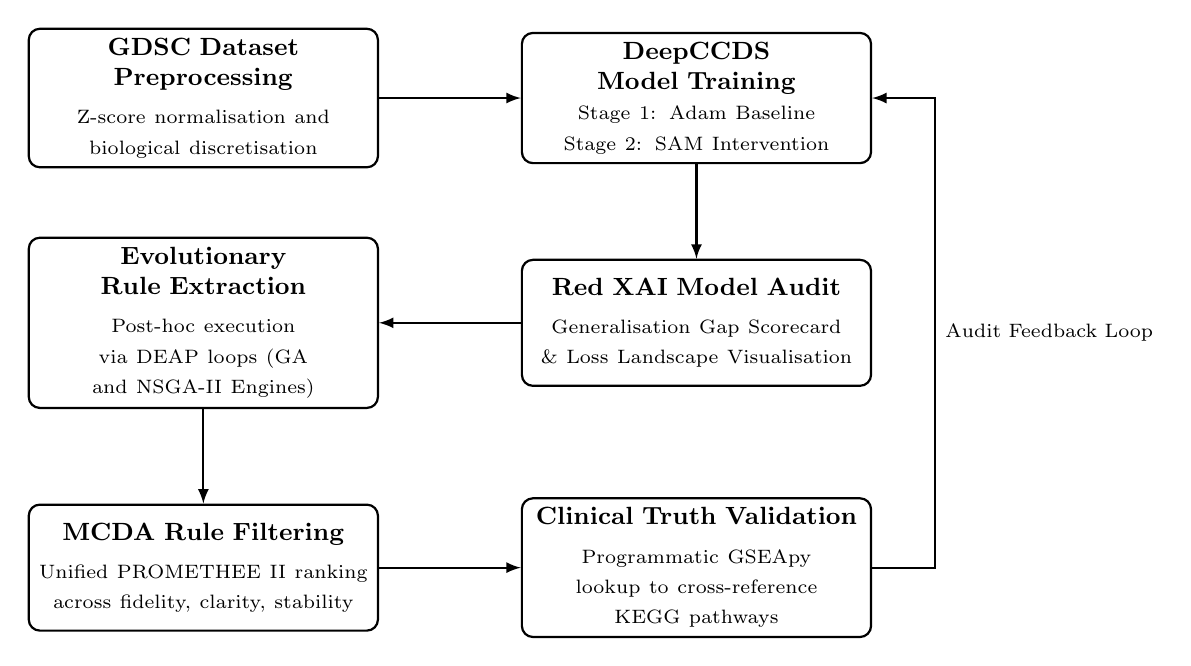
\begin{tikzpicture}[
    node distance=1.2cm and 1.8cm,
    auto,
    block/.style={
        rectangle, 
        draw=black, 
        thick, 
        fill=white,
        text width=4.2cm, 
        align=center, 
        minimum height=1.6cm,
        rounded corners=4pt,
        font=\small
    },
    line/.style={
        draw, 
        -latex, 
        thick
    }
]
    % Nodes setup using explicit positioning parameters to avoid collisions
    \node [block] (data) {
        \textbf{GDSC Dataset Preprocessing}\\
        \vspace{0.1cm}\scriptsize Z-score normalisation and biological discretisation
    };
    
    \node [block, right=of data] (train) {
        \textbf{DeepCCDS Model Training}\\
        \vspace{0.1cm}\scriptsize Stage 1: Adam Baseline\\Stage 2: SAM Intervention
    };
    
    \node [block, below=of train] (audit) {
        \textbf{Red XAI Model Audit}\\
        \vspace{0.1cm}\scriptsize Generalisation Gap Scorecard \& Loss Landscape Visualisation
    };
    
    \node [block, left=of audit] (extract) {
        \textbf{Evolutionary Rule Extraction}\\
        \vspace{0.1cm}\scriptsize Post-hoc execution via DEAP loops (GA and NSGA-II Engines)
    };
    
    \node [block, below=of extract] (mcda) {
        \textbf{MCDA Rule Filtering}\\
        \vspace{0.1cm}\scriptsize Unified PROMETHEE II ranking across fidelity, clarity, stability
    };
    
    \node [block, right=of mcda] (verify) {
        \textbf{Clinical Truth Validation}\\
        \vspace{0.1cm}\scriptsize Programmatic GSEApy lookup to cross-reference KEGG pathways
    };

    % Paths execution with clear directional routing
    \path [line] (data) -- (train);
    \path [line] (train) -- (audit);
    \path [line] (audit) -- (extract);
    \path [line] (extract) -- (mcda);
    \path [line] (mcda) -- (verify);
    
    % Feedback check connection routed safely around the outer edge
    \path [line] (verify.east) -- ++(0.8cm,0) |- node [pos=0.25, right, font=\scriptsize] {
        Audit Feedback Loop
    } (train.east);
\end{tikzpicture}
\caption{Schematic diagram illustrating the proposed closed-loop Red XAI pipeline, charting the 
progression from input data partition interfaces through geometric landscape auditing to multi-criteria 
symbolic selection and programmatic biological verification.}
\label{fig:audit_pipeline_loop}
\end{figure}

\subsubsection{Technical Specifications}
\label{ssub:method_tech_specification}
The end-to-end diagnostic and explanation pipeline is implemented in Python. 
Neural network training routines are driven via PyTorch, while the implementation of 
the single-objective GA and multi-objective NSGA-II rule extraction loops utilises 
the Distributed Evolutionary Algorithms in Python (DEAP) framework. Multi-criteria outranking 
models are executed through the \texttt{pymcdm} library, and automated over-representation 
pathway validation maps are driven via the \texttt{GSEApy} package \cite{Fang2023}. 
\\
Exact software library versions and local hardware parameters will be reported completely at 
the implementation stage to guarantee absolute experimental reproducibility. Due to its dual-step 
gradient update mechanism, the SAM optimiser approximately doubles per-epoch training 
overhead relative to the standard Adam alternative, a factor integrated directly into the 
project milestone timeline. All empirical evaluations enforce the locked 80\% training, 10\% 
validation, and 10\% test data splits outlined in Section \ref{ssub:method_dataset}, 
ensuring that all extracted rule quality scores are computed on identical, uncorrupted validation sets.

\subsection{ANN: Baseline Training and Overfitting Diagnosis}
% -------------------------------------------------------
% ASSIGNED TO: \textcolor{green}{Person 1}
% -------------------------------------------------------
% INSTRUCTION: Paste existing Sections 4.1 through 4.1.5 here.
% Fill the two placeholder values:
%   - Patience parameter (Section 4.1.4)
%   - Domain-specific threshold from Partin et al. or Wu et al. (Section 4.1.4)
% Convert first-person to third person throughout.
% -------------------------------------------------------

% [Paste Section 4.1 Pipeline Overview here]
% [Paste Section 4.1.1 ANN: Baseline Training and Overfitting Diagnosis here]
% [Paste Section 4.1.2 Model Selection: DeepCCDS here]
% [Paste Section 4.1.3 Dataset and Preprocessing Interface here]
% [Paste Section 4.1.4 Stage 1: Training the Overfitting Baseline here]
%   -- FILL: patience parameter placeholder
%   -- FILL: domain-specific threshold placeholder
% [Paste Section 4.1.5 Confirming the Clever Hans Baseline here]

\subsection{Genetic Algorithms for Rule Extraction}
% -------------------------------------------------------
% ASSIGNED TO: \textcolor{green}{Person 2}
% -------------------------------------------------------
% INSTRUCTION: Paste existing Sections 4.2 through 4.2.5 here.
% Fill the run count placeholder (Section 4.2.5 / 4.3).
% Convert first-person to third person throughout.
% -------------------------------------------------------

% [Paste Section 4.2 Genetic Algorithms for Rule Extraction here]
% [Paste Section 4.2.1 Preparation for Rule Extraction here]
% [Paste Section 4.2.2 Pre-processing Data for Rule Extraction here]
% [Paste Section 4.2.3 Implementation of GA via DEAP here]
% [Paste Section 4.2.4 Rule Pruning and Population Diversity here]
% [Paste Section 4.2.5 Validation and Execution here]
%   -- FILL: run count placeholder

Rule extraction from the trained baseline model is performed using a Genetic Algorithm implemented via the Distributed Evolutionary 
Algorithms in Python (DEAP) framework. Following the RED XAI philosophy established in Section 3.1.1, the GA is used not merely to 
produce interpretable if-then rules but as a diagnostic tool to expose the decision logic of the overfitted model and evaluate its 
coherence. The extraction process balances fidelity and comprehensibility as competing objectives throughout \cite{Yedjour2024}.
\subsubsection{Preparation for Rule Extraction}
Prior to rule extraction, loss landscape visualisation is applied to the trained baseline model to characterise the sharpness of the 
minima to which it has converged and to document the overfitting behaviour that motivates the SAM intervention in Stage 2. This 
visualisation serves as a qualitative complement to the generalisation gap metric established in Section 4.1.4 and provides a 
geometric baseline against which the SAM-regularised model's landscape is later compared \cite{Li2018}.
\subsubsection{Pre-processing Data for Rule Extraction}
Rather than operating on continuous inputs, rule extraction requires discretisation of the gene expression features. Continuous input 
ranges are divided into k partitions of equal length, producing discrete categories such as high expression, intermediate expression, 
and low expression as described in Section 4.1.3. Rules are then extracted in the format: if X$_1$ is in partition A and X$_2$ is in 
partition 
B, then predicted response Y, where each condition corresponds to a discretised feature partition \cite{Yedjour2024}.
\subsubsection{Implementation of GA via DEAP}
An evolutionary loop is configured within the DEAP framework to discover optimal rule sets. Each individual chromosome in the population 
represents a candidate rule set encoded as a vector, where each element corresponds to a discretised attribute partition or a special 
value of -1 to indicate that the attribute is not involved in the rule \cite{Yedjour2024}.
The fitness function adopts a multi-objective formulation, simultaneously optimising fidelity to the black-box model, predictive accuracy 
on held-out data, and comprehensibility measured by rule length \cite{Yedjour2024}. Tournament selection is used to identify parent 
individuals for reproduction. Two-point crossover combines rule segments from two parent chromosomes to produce offspring, and mutation 
introduces random changes – such as adding or removing a condition – to maintain population diversity and prevent premature convergence 
on local optima \cite{Yedjour2024}.
\subsubsection{Rule Pruning and Population Diversity}
Following each generation, rule pruning is applied to remove conditions with low confidence and support, maintaining a concise rule set 
and reducing rule explosion. Aging evolution is additionally applied as a diversity mechanism to prevent the population from converging 
prematurely on local optima, ensuring that the evolutionary search continues to explore the rule space rather than stagnating on a 
suboptimal solution \cite{Yedjour2024}.
\subsubsection{Validation and Execution}
The GA is executed for 50 generations with a population size of 35 to 45 individuals, following the configuration established by 
\cite{Yedjour2024}. The output of each run is a Pareto front representing a set of non-dominated rule sets that each reflect a 
different trade-off between fidelity and comprehensibility. The final selected rule set is the one that achieves the best balance 
across these objectives as determined by PROMETHEE II ranking in Section 4.5.1. 
\\
\textcolor{red}{To account for the stochastic nature of the genetic algorithm, rule extraction is
repeated across 30 independent runs, each initialised with a different random seed. The non-dominated
rule sets produced across all runs are aggregated into a single rule pool for the given model condition,
which is then ranked using PROMETHEE II (Section 4.5.1). This ensures the final ranked rules reflect
structure that is consistent across runs rather than the product of a single stochastic search. The
choice of 30 runs follows standard practice for the statistical comparison of stochastic optimisation
algorithms \cite{Derrac2011} and is provisional, subject to confirmation against the protocol of
\cite{Yedjour2024} and the project timeline.}

\subsection{NSGA-II for Rule Extraction}
% -------------------------------------------------------
% ASSIGNED TO: \textcolor{green}{Person 3}
% -------------------------------------------------------
% INSTRUCTION: Paste existing Section 4.3 NSGA-II content here.
% Convert first-person to third person throughout.
% -------------------------------------------------------

% [Paste Section 4.3 NSGA-II here]

\subsection{SAM Regularisation}
% -------------------------------------------------------
% ASSIGNED TO: \textcolor{green}{Person 4}
% -------------------------------------------------------
% INSTRUCTION: Paste existing Sections 4.4 through 4.4.3 here.
% Convert first-person to third person throughout.
% -------------------------------------------------------

% [Paste Section 4.4 SAM Regularisation here]
% [Paste Section 4.4.1 Intervention Objective here]
% [Paste Section 4.4.2 SAM Optimisation Mechanism here]
% [Paste Section 4.4.3 Expected Effect on Generalisation here]
The second stage of the experimental pipeline retrains the DeepCCDS architecture using the Sharpness-Aware Minimisation (SAM) 
optimiser to reduce the generalisation gap and improve loss landscape smoothness.

\subsubsection{Intervention Objective}
SAM is applied to the same DeepCCDS architecture, dataset splits, preprocessing pipeline, and training configuration used in the baseline 
model, ensuring that the optimisation strategy is the sole variable distinguishing the two models. This controlled substitution 
isolates the effect of loss landscape geometry on three downstream outcomes: the generalisation gap, the smoothness of the loss 
landscape as measured through visualisation, and the quality of rules extracted by the evolutionary algorithms in Sections 4.2 and 4.3.

\subsubsection{SAM Optimisation Mechanism}
SAM modifies the standard training objective by introducing a neighbourhood-based perturbation step. Rather than minimising the loss 
at the current parameters $\theta$ alone, the optimiser evaluates the worst-case loss within a local $\epsilon$-ball around the current weights, 
effectively minimising the loss at perturbed parameters $\theta + \epsilon$. This forces the model to favour solutions that remain stable under 
small parameter perturbations, penalising sharp curvature in the loss surface and encouraging convergence toward flat minima 
\cite{Foret2021,Li2018}.

\subsubsection{Expected Effect on Generalisation}
The baseline model is characterised by high training performance, lower validation performance, and a large generalisation gap, indicating 
that the model has memorised training-specific noise rather than learning stable biological patterns. By converging on flatter minima, 
the SAM-regularised model is expected to reduce the training-validation discrepancy, producing more balanced performance across both 
sets. Following \cite{Springer2024}, this improvement in generalisation is expected to produce more balanced feature representations, 
which in turn should yield extracted rules with fewer spurious conditions and higher biological coherence than those produced by the 
baseline model.


\subsection{Evaluation Strategy}
% -------------------------------------------------------
% ASSIGNED TO: \textcolor{green}{Person 5}
% -------------------------------------------------------
% INSTRUCTION: Paste existing Sections 4.5 through 4.5.3 here.
% ADD the new SOTA baseline comparison subsection (marked in red below).
% Convert first-person to third person throughout.
% -------------------------------------------------------

% [Paste Section 4.5 Evaluation Strategy here]
% [Paste Section 4.5.1 Multi-Criteria Ranking via PROMETHEE II here]
% [Paste Section 4.5.2 Statistical Significance (Wilcoxon Signed-Rank Test) here]
% [Paste Section 4.5.3 Automated Biological Verification (GSEApy) here]

The evaluation strategy employs a Multi-Criteria Decision Analysis (MCDA) framework to objectively rank the extracted rules, moving 
beyond a single-metric (accuracy-based) approach \cite{Matejova2025}.

\subsubsection{Multi-Criteria Ranking via PROMETHEE II}
To determine the top 10 rules from the thousands generated by the genetic algorithm, the PROMETHEE II method will be implemented using the 
pymcdm library \cite{Yedjour2024}. Each rule is treated as an alternative and ranked based on three conflicting criteria:
\\
Fidelity: Measured using the F1-score of the rule’s predictions compared to the black-box model’s predictions. This ensures that the rule 
acts as a faithful surrogate \cite{Guidotti2021}.
\\
Comprehensibility: Measured by the Length of the Rule (i.e.,number of conditions). Shorter rules are prioritised to avoid rule explosion 
\cite{Yedjour2024}.
\\
Stability: Calculated by the variance in rule performance across different cancer types in the GDSC dataset \cite{Ye2024}.
\\
\textcolor{red}{For any comparison between two rule sets (for example, baseline versus SAM-regularised,
or evolutionary versus decision-tree extraction), all rules entering that comparison are ranked within a
single combined PROMETHEE II run. This ensures each rule's net outranking flow is computed against a
common reference set, so that the resulting $\phi$ values are directly comparable before the
Mann--Whitney U test is applied. Ranking each rule set in a separate run would render the flows
incommensurable, as PROMETHEE net flows are defined only relative to the alternatives present in a given
run.}
\subsubsection{Statistical Significance \textcolor{red}{(Mann--Whitney U Test)}}
\textcolor{red}{To confirm that differences in rule quality between the baseline and SAM-regularised
models are statistically significant rather than coincidental, a Mann--Whitney U test (equivalently,
the Wilcoxon rank-sum test) is applied to the net outranking flows of the top 10 baseline rules and the
top 10 SAM rules, drawn from the common PROMETHEE II run described above. The Mann--Whitney U test is appropriate because the baseline and
SAM-regularised rule sets comprise distinct rules with no natural one-to-one correspondence; they
therefore constitute two independent samples rather than matched pairs, for which a paired test such
as the Wilcoxon signed-rank test would be inappropriate. A non-parametric test is required because the
distribution of net outranking flows is bounded, derived from a small sample, and cannot be assumed to
follow a normal distribution \cite{Derrac2011}. A $p$-value threshold of 0.05 is used to determine statistical
significance; a result below this threshold is interpreted as evidence that the difference in rule
quality between the baseline and SAM conditions is unlikely to be due to random chance.}

\subsubsection{Automated Biological Verification (GSEApy)}
The genes identified in the top-ranked rules from both the baseline and SAM-regularised models are submitted to over-representation 
analysis using the GSEApy library \cite{Fang2023}, which provides a programmatic interface to the Enrichr and KEGG pathway databases. 
For each rule set, GSEApy tests whether the genes appearing in the extracted rules are statistically enriched in known biological pathways 
relative to a background gene set. The pathway enrichment p-value is used to determine whether the rules align with established oncogenic 
mechanisms, such as apoptosis or DNA repair pathways, or whether they represent statistically arbitrary associations with no biological 
grounding \cite{Subramanian2005}. A significantly higher enrichment score in the SAM-regularised rule set relative to the baseline 
would constitute evidence that improved generalisation produces not only statistically better rules but biologically more meaningful 
ones, directly addressing sub-research question 4 from Section 2.


% -------------------------------------------------------
% NEW CONTENT REQUIRED — SOTA BASELINE COMPARISON
% (Supervisor feedback: compare our method to SOTA approaches)
% -------------------------------------------------------

\subsubsection{SOTA Baseline Comparison: Decision Tree Rule Extraction}

\textcolor{red}{
% ADD: Decision tree as a SOTA rule extraction baseline.
% This is the cleanest way to satisfy the supervisor's request to compare to SOTA
% without adding entirely new algorithm implementations.
% Suggested text:
To contextualise the quality of rules produced by the GA and NSGA-II pipelines, a CART
decision tree \cite{Breiman1984} is included as a deterministic rule extraction baseline,
representing the most widely adopted alternative to evolutionary rule extraction in the XAI
literature \cite{Arrieta2020}. The decision tree is fitted to the predictions of both the baseline
and SAM-regularised DeepCCDS models using scikit-learn, with maximum depth constrained to
prevent rule explosion. Rules are extracted from the fitted tree and evaluated under the identical
PROMETHEE II framework described in Section 4.5.1, using the same fidelity, comprehensibility,
and stability criteria. This enables a direct comparison between deterministic surrogate-based
rule extraction and the proposed evolutionary approach across both model conditions. \textcolor{red}{The Mann--Whitney U test described in Section~\ref{subsec:statsig} is applied to the
PROMETHEE outranking flow distributions of the decision tree rules and the GA/NSGA-II rules to
determine whether the improvement from evolutionary extraction is statistically significant, and
whether this advantage is maintained after SAM regularisation.}
% NOTE: Breiman et al. (1984) "Classification and Regression Trees" is the standard CART citation.
% Add to references.bib: Breiman, L., Friedman, J., Stone, C.J., Olshen, R.A. (1984).
% Classification and Regression Trees. CRC Press.
}

\subsection{Experiments}
% -------------------------------------------------------
% ASSIGNED TO: \textcolor{green}{Person 5}
% -------------------------------------------------------
% INSTRUCTION: Paste existing Section 4.6 Experiments here.
% ADD the CCLE robustness validation paragraph (marked in red below).
% Convert first-person to third person throughout.
% -------------------------------------------------------

% [Paste Section 4.6 Experiments here]
The research follows a two-stage experimental design to isolate the impact of model sharpness on explanation quality.
In Stage 1, the Overfitting Baseline is established as the RED XAI diagnostic starting point. DeepCCDS is trained using the Adam 
optimiser until a stable generalisation gap has emerged using the early stopping criterion defined in Section 4.1.4, confirming the 
Clever Hans baseline. Rules are then extracted from this overfitted model by both the GA and NSGA-II pipelines. The resulting rule sets 
are audited using PROMETHEE II ranking and GSEA pathway enrichment analysis to document the Fragility Baseline scorecard.
In Stage 2, the Regularisation Intervention is applied. The same DeepCCDS architecture is retrained using the SAM optimiser to smooth the 
loss landscape and reduce the generalisation gap, as described in Section 4.4. Rules are re-extracted using identical GA and NSGA-II 
parameters to ensure comparability. The same PROMETHEE II and GSEA audit is performed to generate a second evaluation scorecard. 
Wilcoxon signed-rank tests are then applied to the distributions of PROMETHEE outranking flows from both stages to determine whether 
the improvement in rule quality is statistically significant.


% -------------------------------------------------------
% NEW CONTENT — SECOND DATASET FOR ROBUSTNESS (supervisor suggestion)
% -------------------------------------------------------

\textcolor{red}{
% ADD: CCLE as a planned robustness validation dataset.
% The supervisor suggested this if time permits. Frame it as a stretch objective.
% Suggested text:
\paragraph{Robustness Validation: Cancer Cell Line Encyclopedia (CCLE)}
As a stretch objective, subject to timeline constraints, the complete RED XAI pipeline will be
applied to a second pharmacogenomic dataset: the Cancer Cell Line Encyclopedia (CCLE)
\cite{Barretina2012}. The CCLE provides gene expression profiles and drug response data for
cancer cell lines using a structurally compatible format to GDSC, and has been used alongside
GDSC in several of the studies cited in this proposal \cite{Partin2023, Baptista2021}. Applying
the pipeline to CCLE data, with LN IC\textsubscript{50} as the response target, would enable
assessment of whether the observed advantage of SAM regularisation over the Adam baseline
in terms of rule fidelity, comprehensibility, and biological validity generalises beyond the GDSC
dataset. Consistent results across both datasets would substantially strengthen the robustness
of the study's conclusions. No new statistical machinery is required; the same Wilcoxon
signed-rank test and PROMETHEE II framework are applied, and results are reported
comparatively.
% NOTE: Barretina et al. (2012) "The Cancer Cell Line Encyclopedia enables predictive modelling
% of anticancer drug sensitivity." Nature, 483, 603-607. Add to references.bib.
}

\subsection{Expected Results}

Four primary outcomes are anticipated from this methodology.
First, an inverse correlation is expected between the generalisation gap and rule comprehensibility: the SAM-regularised model should 
produce rules with fewer conditions than the baseline while maintaining comparable fidelity, consistent with the hypothesis that flatter 
minima yield more balanced feature representations \cite{Springer2024}.
\\\\
Second, the rules extracted from the SAM-regularised model are expected to show higher stability scores across different cancer subtypes 
in the GDSC dataset, reflecting the capture of genuine biological signal rather than training-specific noise.
\\\\
Third, the genes appearing in SAM-optimised rules are expected to show statistically significant enrichment in established KEGG pathways 
(p < 0.05) compared to baseline rules, providing biological grounding for the claim that regularisation improves not only statistical but 
clinical rule quality.
\\\\
Fourth, and contingent on the preceding outcomes, the study aims to demonstrate that the generalisation gap serves as a reliable 
diagnostic indicator of explanation fragility, and that SAM regularisation constitutes an effective intervention for improving the 
fidelity, comprehensibility, and biological validity of symbolically extracted rules in cancer pharmacogenomics.


\section{Planning}
% -------------------------------------------------------
% ASSIGNED TO: \textcolor{green}{Person 1} (or whoever has the Gantt chart)
% -------------------------------------------------------
% INSTRUCTION: Replace the placeholder below with a proper Gantt chart.
% Use the pgfgantt package (already compatible with the preamble style).
% The existing chart image in the PDF can be recreated in LaTeX or
% inserted as a figure if exported from another tool.
% -------------------------------------------------------

\textcolor{red}{
% URGENT: Replace this placeholder with the actual Gantt chart before submission.
% The current proposal has a red-text placeholder visible in the document.
% Suggested approach: use the pgfgantt LaTeX package, or export from Excel/GanttProject
% and include as \includegraphics.
}

The project is structured across six months from June to November 2026. All five team members
begin with shared boilerplate and pilot testing in June to establish a common codebase and verify
the pipeline end-to-end. Data preparation and baseline model training are completed in July.
Rule extraction by Persons 2 and 3, alongside the SAM intervention by Person 4, run in
parallel across August and September. Person 5 conducts PROMETHEE II ranking, statistical
validation, and biological verification on a rolling basis from August through October as rule
sets are produced. Final evaluation, comparative analysis, and report writing are completed
across October and November by all team members.

% [INSERT GANTT CHART FIGURE HERE]

\bibliographystyle{plain}
% \bibliography{alpha} - was giving weird labelling instead of numbers - switching to plain
\bibliography{references}

\end{document}